%%%%%%%%%%%%%%%%%%%%%%%%%%%%%%%%%%%
\subsection{Cameras}
\label{sec:fdsp-slow-cryo-cameras}
% glenn, jim s, chuck


% % % %
\subsubsection{Cryogenic Cameras (cold)}

% % % %
\subsubsection{Inspection Cameras (warm)}

% % % %
\subsubsection{Light emitting system}
%%% same text as dual-phase
The light emitting system will be based on Light-Emitting Diodes (LEDs),
with the capability of illuminating interior with selected wavelengths
(IR and visible) that are suitable for detection by the CCD cameras.
Performance criteria for the light emission system are based on the
efficiency of detection with the cameras, in conjunction with adding
minimal heat to the cryostat. The use of very high efficiency LEDs will
assist with the goal of reducing heat generation; as an exmple, one
\SI{750}{nm}
red LED has a specification of 32\%\ conversion of
electrical input power to light. 

While data on the performance of LEDs at cryogenic temperatures is sparse,
there are some studies related to NASA projects\cite{Carron:2017zzz}, which
indicate that LED efficiency increases with reduced temperature,
and that the emitted wavelengths may change, particularly for ``blue'' LEDs,
but the wavelength changes cited would have no impact on illumination.

\begin{dunefigure}[LED chain for illumination]{fig:sp-cisc-LEDs}
  {Suggested LED chain for lighting inside the cryostat, with
    dual-wavelength and failure-tolerant operation.}
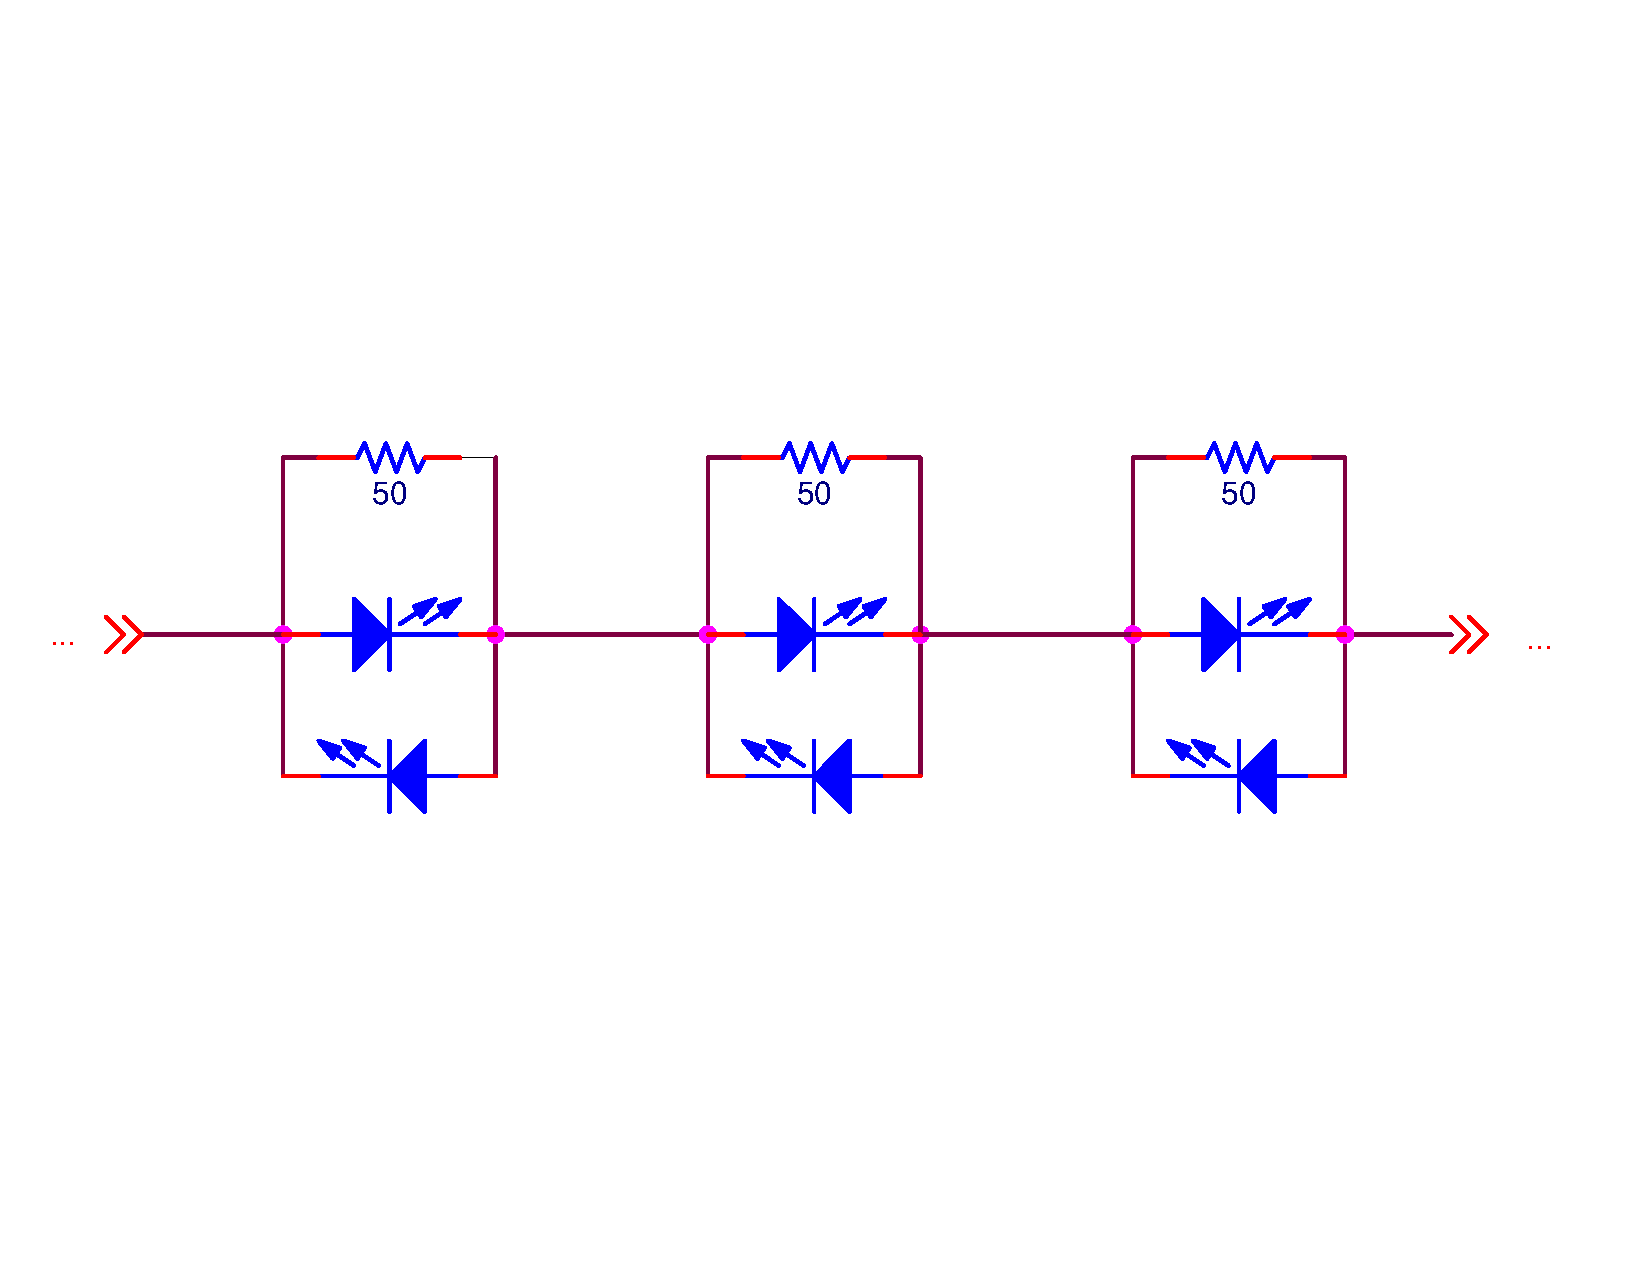
\includegraphics[width=0.8\textwidth]{figures/CISC-Lighting.pdf}
\end{dunefigure}

A `chain' of LEDs should be connected in series and driven with a
constant-current circuit. It would be advantageous to pair each
LED in parallel with an opposite polarity LED and a resistor
(see Fig.~\ref{fig:sp-cisc-LEDs}).
This allows two different wavelengths of illumination with a single installed
chain (by changing the direction of the drive current) and 
continued use of an LED chain even if individual LEDs have failed.
Installation of multiple LED chains will also mitigate device failures,
and will be necessary for full illumination of the detector.
